\chapter{Same-sign dilepton final state}

Almost every new (or rare SM) physics analysis relies on a ``killer'' variable
or technique
to differentiate signal from background and increase the signal-to-noise
ratio to a level that is conducive to further interpretation.
The technique used in this thesis exploits the fact that seeing a pair of leptons
with the same charge as a product of proton-proton collision processes
(e.g., $\PW$/$\PZ$ production, QCD) is very, very rare,
but is quite common in scenarios of new (or rare SM) physics.

We start by examining the rare production of four top quarks (\tttt) in the SM,
as SUSY processes follow
similar patterns and will be dicussed in more detail in the subsequent section.
The four top quarks of SM \tttt will each decay into a \PQb quark and \PW boson.
A \PW boson decays into a charged lepton and matching neutrino 
($e\bar\nu_e$, $\mu\bar\nu_\mu$, $\tau\bar\nu_\tau$) approximately 1/3 probability.
For four \PW bosons ($\PW^+\PW^+\PW^-\PW^-$), the lepton multiplicities and characteristics are summarized in
Fig~\ref{fig:fourtoppie}. Up to 12\% of SM \tttt can be selected by requiring
a same-sign (SS) dilepton in the final state. 

Turning to background SM processes, to first order, requiring two leptons
(SS or not) eliminates QCD processes  with only quarks/gluons (u, d, s, c, b, g) in the final state.
Figure~\ref{fig:SMxsecs} summarizes
CMS measurements of many other SM processes.
Three of the highest cross section processes 
are $\PW$, $\PZ$, and $\ttbar$, which give one lepton or two opposite sign leptons.
In fact, continuing down the mountain, the first process that can give prompt
SS dileptons is $\PW\PZ$. Thus, the SS dilepton selection is an effective
``cut'' that rejects processes above $\mathrm{O}(10)\unit{pb}$. Compared to many other
search strategies, which exploit extreme event kinematics, the SS dilepton selection allows probing softer
events with less transverse momenta and missing transverse energy.




\begin{figure}[!hbtp]
\centering
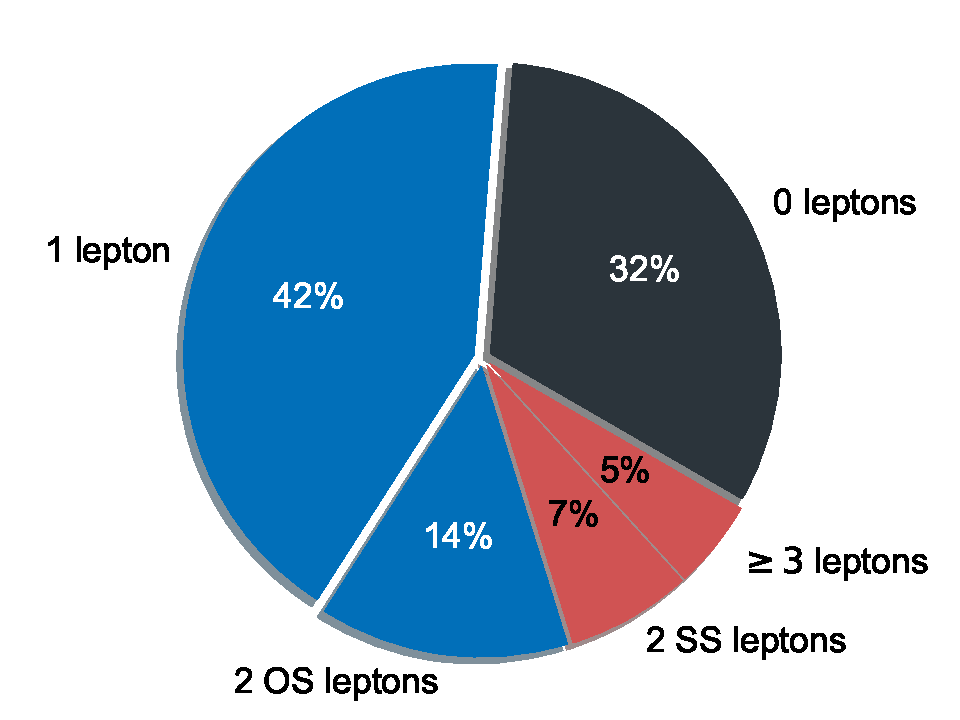
\includegraphics[width=.50\textwidth]{figs/misc/fourtopdecay_pie.pdf} \\
\caption{Lepton multiplicities of four $\PW$ final states.}
\label{fig:fourtoppie}
\end{figure}

\begin{figure}[!hbtp]
\centering
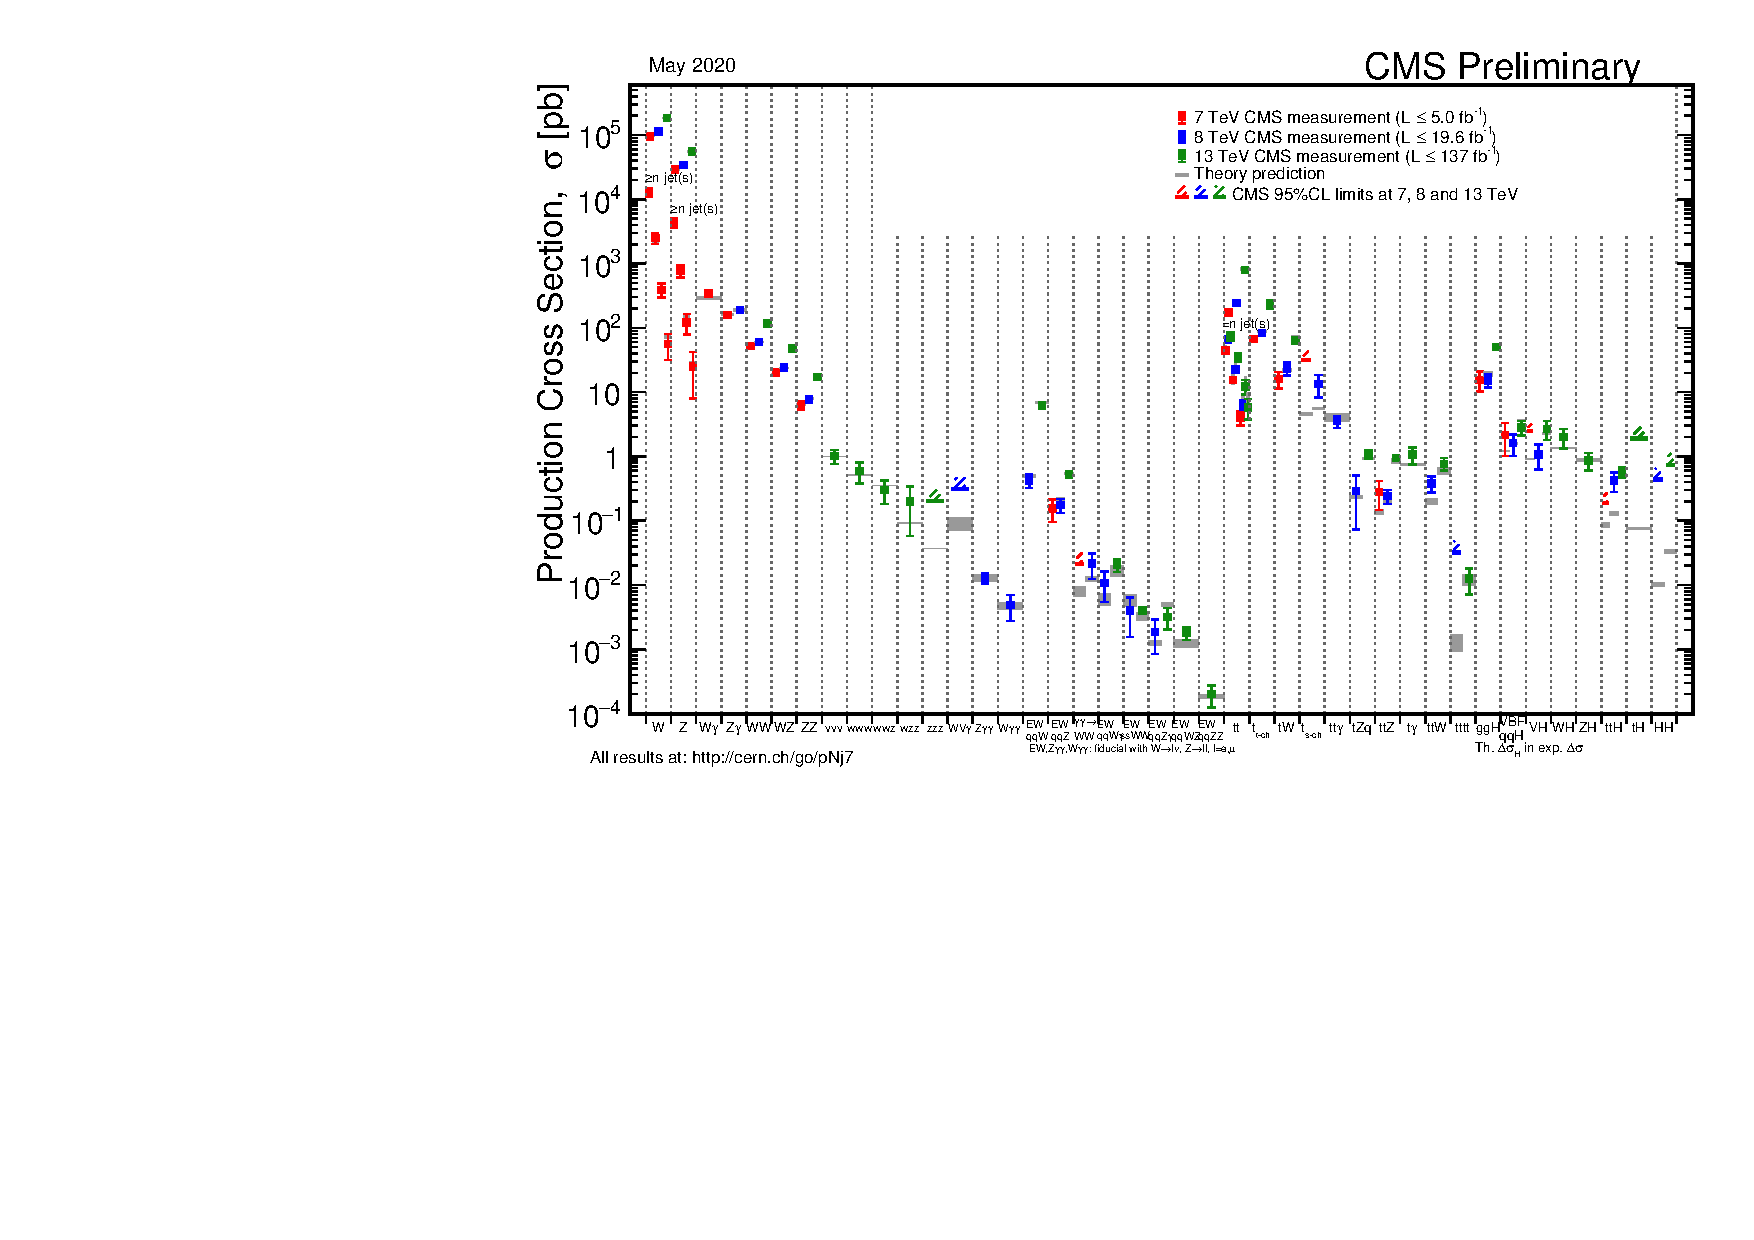
\includegraphics[width=.95\textwidth]{figs/misc/sm_xsecs.pdf} \\
\caption{Summary of SM cross section measurements at CMS~\cite{CMS:SMxsecs}.
(Spoiler alert: the results presented later in this thesis correspond to one
of the points in this plot!)
}
\label{fig:SMxsecs}
\end{figure}

\FloatBarrier

\section{SUSY processes}


Many SUSY models with strong pair production mechanisms result in
final states with a number of leptons, ideal for SS final states.
Cross sections of pair production models with gluinos and squarks 
are shown in Fig.~\ref{fig:susy_xsecs}, and are as low as a few \fbinv 
for gluino/squark masses between 1.5\TeV and 2\TeV.

\begin{figure}[htb!]
    \centering
    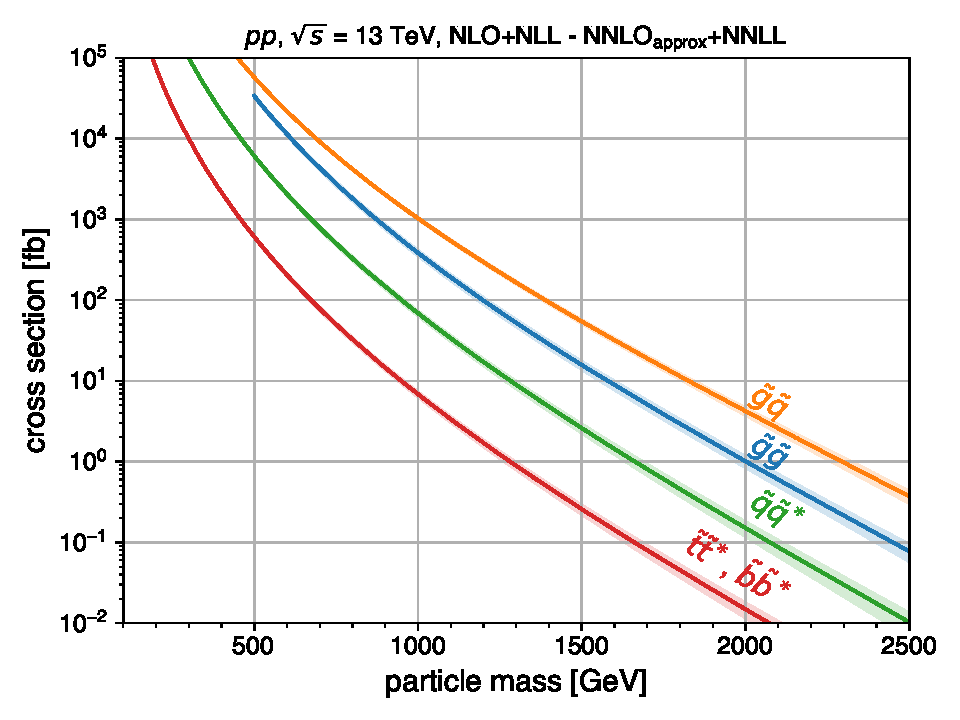
\includegraphics[width=0.75\textwidth]{figs/ssan/plot_susy_xsecs}
\caption{Strong production cross sections for SUSY processes at the LHC. Calculations from \cite{THEORY:SUSYxsecs}.}
\label{fig:susy_xsecs}
\end{figure}

Gluino pair production models giving rise to signatures with up to four \cPqb\
quarks and \PW\ bosons are shown in Fig.~\ref{fig:susy_diag_set1}. In
these models, the gluino decays to the lightest squark ($\gluino \to \susyq
\cPq$), which then decays to same-flavor ($\susyq \to \cPq \lsp$) or
different-flavor ($\susyq \to \cPq' \chiplmin$) quarks. The chargino
($\chiplmin$) decays to a \PW\ boson and a neutralino ($\lsp$) via $\chiplmin
\to \PW^{\pm} \lsp$, where the \lsp is taken to be the lightest stable SUSY (LSP)
particle and is not directly detectable.

The first scenario, displayed in Fig.~\ref{fig:susy_diag_set1}a and denoted
\Totttt, includes an off-shell top squark ($\susytop$) leading to a
three-body decay of the gluino, $\gluino \to \ttbar\lsp$, and resulting in events
with four \PW\ bosons and four \cPqb\ quarks. This topology is thus similar
to SM \tttt with the addition of missing energy from the LSP.
Figure~\ref{fig:susy_diag_set1}b presents a similar model (\TfttbbWW) but where
the gluino decay results in a chargino that decays into a neutralino
and a \PW\ boson. The model shown in Fig.~\ref{fig:susy_diag_set1}c (\Tftttt)
is identical to \Totttt except that the intermediate top squark is on-shell.
The mass splitting between the $\susytop$ and the \lsp is taken to be
$m_{\susytop} - m_{\lsp} = m_{\cPqt}$, where $m_{\cPqt}$ is the top quark
mass. This mass splitting corresponds to a challenging region of parameter
space for the observation of the $\susytop \to \cPqt \lsp$ decay. The model
of Fig.~\ref{fig:susy_diag_set1}d (\Tfttcc) is identical to 
\Tftttt except that the $\susytop$ decay involves a \PQc quark. In
Fig.~\ref{fig:susy_diag_set1}e, the process includes a virtual
light-flavor squark, leading to three-body decays of $\gluino \to \cPq \cPq'
\chiplmin$ or $\gluino \to \cPq \cPq' \neutralinotwo$, with a resulting
signature of two \PW\ bosons, two \PZ\ bosons, or one of each (the case shown
in Fig.~\ref{fig:susy_diag_set1}e), and four light-flavor jets. This model,
\TfqqqqWZ, with a resulting signature of one \PW\ boson and one \PZ\ boson,
is considered separately for two different assumptions of the chargino mass,
$m_{\chiplmin} = 0.5(m_{\gluino} + m_{\lsp})$, and $m_{\chiplmin} =
m_{\lsp}+20 \GeV$, producing on- and off-shell bosons, respectively. The
model is also considered with the assumption of decays to two \PW\ bosons (\TfqqqqWW).

Figure~\ref{fig:susy_diag_set2}a shows a model of bottom squark production and decay
via $\sbottomone \to \cPqt \chiplmin$, giving two \cPqb\
quarks and four \PW\ bosons. This model, \TsttWW, is considered as a function
of the the lightest bottom squark, $\sbottomone$, and \chiplmin masses. The
\lsp mass is fixed at 50\GeV, which results in two off-shell \PW\ bosons 
when the \chiplmin mass is less than approximately
130\GeV. Figure~\ref{fig:susy_diag_set2}b displays the \TsttHZ model
with top squark pair production and a subsequent decay of
$\susytoptwo\to\susytopone\PH/\PZ$, with $\susytopone \to \cPqt\lsp$,
producing signatures with two \PH\ bosons, two \PZ\ bosons, or one of each.
In this model the \lsp mass is fixed such that
$m(\susytopone)-m(\lsp)=m_{\cPqt}$.

The R parity violating (RPV) decays considered in the SUSY analysis are \ToqqqqL
(Fig.~\ref{fig:susy_diag_set3}a) and \Totbs (Fig.~\ref{fig:susy_diag_set3}b). In
\ToqqqqL, the gluino decays to the lightest squark ($\gluino \to \susyq
\cPq$), which decays to a quark ($\susyq \to \cPq \lsp$)
with an off shell $\lsp$ decaying into two quarks and a charged
lepton, giving rise to a prompt 5-body decay of the gluino. In the \Totbs model, the
gluinos each decay into three different SM quarks ($\PQt$, $\PQb$, and $\PQs$).

\begin{figure}[htb!]
    \centering
    \subfloat[T1tttt]{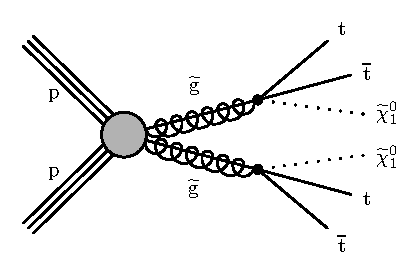
\includegraphics[width=0.48\textwidth]{figs/ssp/diag_T1tttt}}
    \subfloat[T5ttbbWW]{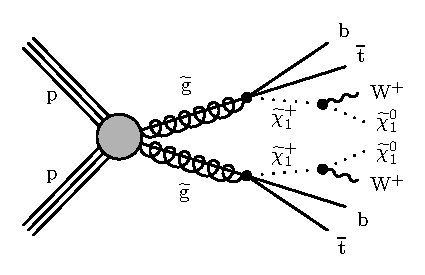
\includegraphics[width=0.48\textwidth]{figs/ssp/diag_T5ttbbWW}} \\
    \subfloat[T5tttt]{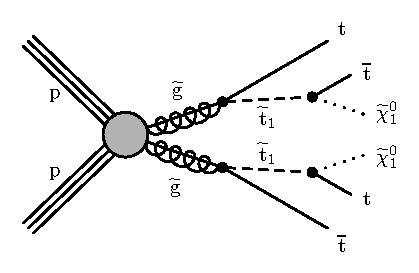
\includegraphics[width=0.48\textwidth]{figs/ssp/diag_T5tttt}}
    \subfloat[T5ttcc]{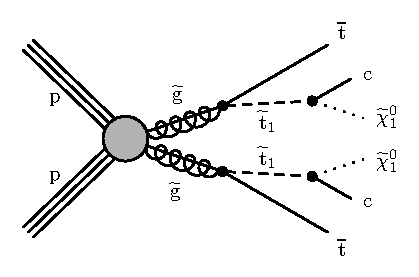
\includegraphics[width=0.48\textwidth]{figs/ssp/diag_T5ttcc}} \\
    \subfloat[T5qqqqWZ]{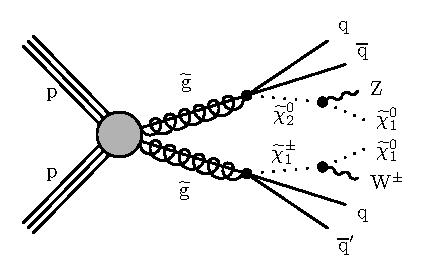
\includegraphics[width=0.48\textwidth]{figs/ssp/diag_T5qqqqWZ}}
\caption{Diagrams illustrating the simplified RPC SUSY models with gluino production considered in this analysis.}
\label{fig:susy_diag_set1}
\end{figure}

\begin{figure}[htb!]
    \centering
    \subfloat[T6ttWW]{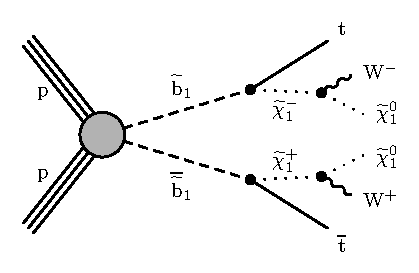
\includegraphics[width=0.48\textwidth]{figs/ssp/diag_T6ttWW}}
    \subfloat[T6ttHZ]{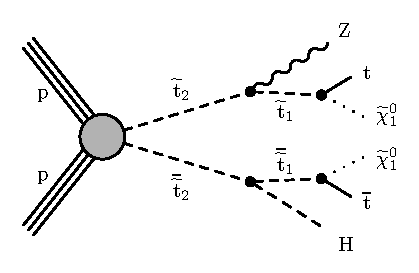
\includegraphics[width=0.48\textwidth]{figs/ssp/diag_T6ttHZ}} \\
\caption{Diagrams illustrating the simplified RPC SUSY models with squark production considered in this analysis.}
\label{fig:susy_diag_set2}
\end{figure}

\begin{figure}[htb!]
    \centering
    \subfloat[T1qqqqL]{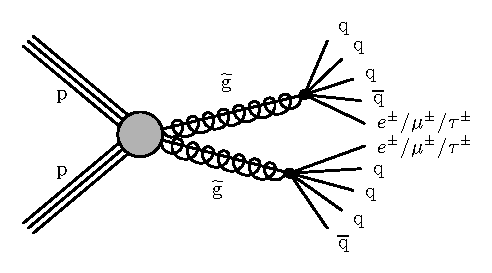
\includegraphics[width=0.53\textwidth]{figs/ssp/diag_T1qqqqL}}
    \subfloat[T1tbs]{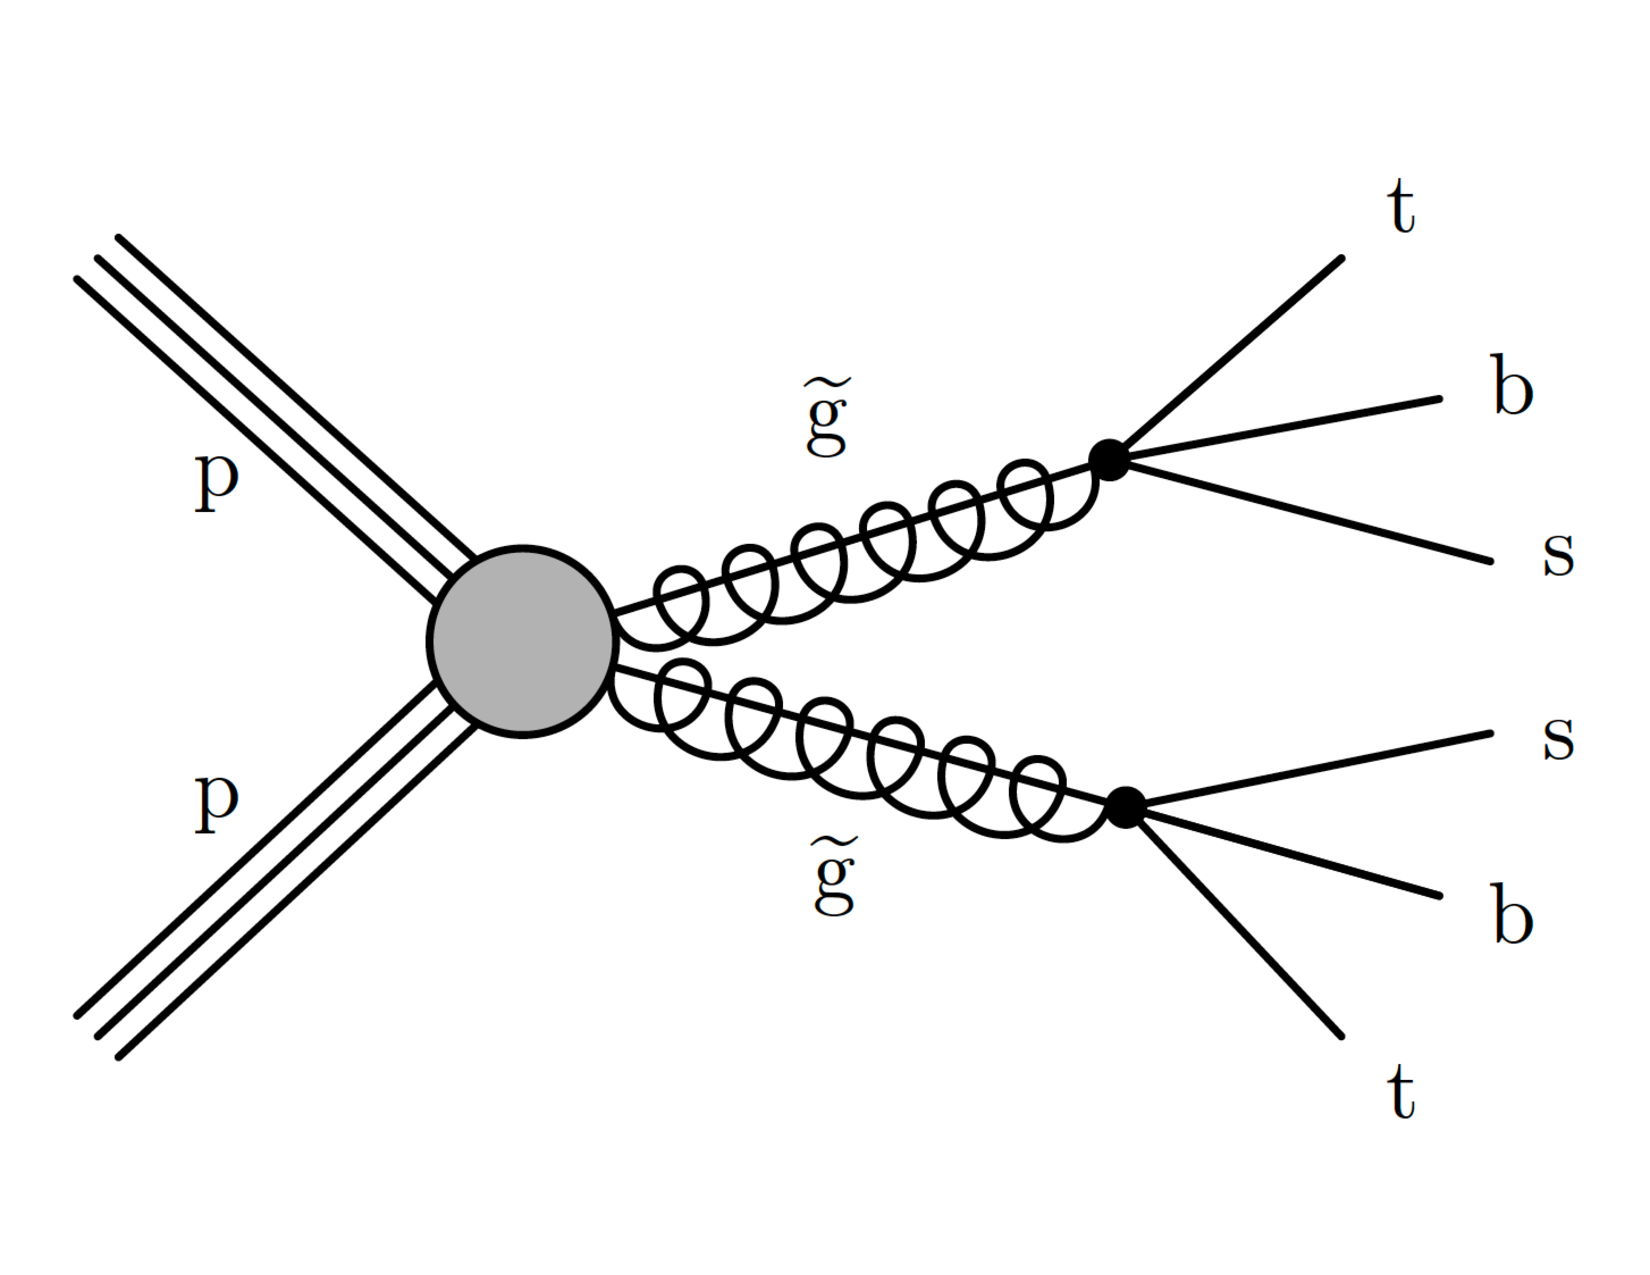
\includegraphics[width=0.45\textwidth]{figs/ssp/diag_T1tbs}} \\
\caption{Diagrams illustrating the two simplified RPV SUSY models considered in this analysis.}
\label{fig:susy_diag_set3}
\end{figure}

A summary of the 14 simplified SUSY models considered in the inclusive SUSY analysis
is shown in Table~\ref{tab:susyprocesses}. The last few columns give final state multiplicities
of bosons and \PQb quarks. At a glance, based on the high multiplicity of $\PW$ and $\PZ$ bosons,
it is clear that these models result in SS final states and many jets.

\begin{table} [h!]
\begin{center}
\resizebox{0.99\textwidth}{!}{
{\renewcommand{\arraystretch}{1.85}
\begin{tabular}{l|p{0.4\textwidth}cccccccc}
\hline
Model & Process & Constraint & Mass 1 & Mass 2 & RPV & \#W & \#Z & \#H & \#b\\
\hline
\Totttt & $\gluino\to\ttbar\lsp$ & \NA & $m_{\gluino}$ & $m_{\lsp}$ & \NA  & 4 & 0 & 0 & 4 \\
\TfttbbWW & $\gluino\to\cPqt\cPqb\chiplmin$ & $m_{\chiplmin}=m_{\lsp}+5\GeV$ & $m_{\gluino}$ & $m_{\lsp}$ & \NA & 4 & 0 & 0 & 4 \\
\Tftttt & $\gluino\to\susytopone\cPqt$, $\susytopone\to\cPqt\lsp$ & $m_{\susytop}-m_{\lsp}=m_{\PQt}$ & $m_{\gluino}$ & $m_{\lsp}$ & \NA  & 4 & 0 & 0 & 4 \\
\Tfttcc & $\gluino\to\susytopone\cPqt$, $\susytopone\to\cPqc\lsp$ & $m_{\susytop}-m_{\lsp}=20\GeV$&  $m_{\gluino}$ & $m_{\lsp}$ & \NA  & 2 & 0 & 0 & 2 \\
\TfqqqqWW & $\gluino\to\cPq\cPq'\chiplmin$, $\chiplmin\to\PW^{\pm}\lsp$ & $m_{\chiplmin}=0.5(m_{\gluino}+m_{\lsp})$ & $m_{\gluino}$ & $m_{\lsp}$ & \NA  & 2 & 0 & 0 & 0 \\
\TfqqqqWW & $\gluino\to\cPq\cPq'\chiplmin$, $\chiplmin\to\PW^{\pm}\lsp$ & $m_{\chiplmin}=m_{\lsp}+20\GeV$ & $m_{\gluino}$ & $m_{\lsp}$ & \NA  & 2 & 0 & 0 & 0 \\
\TfqqqqWZ & $\gluino\to\cPq\cPq'(\chiplmin/\neutralinotwo)$, \newline $\chiplmin\to\PW^{\pm}\lsp$, $\neutralinotwo\to\PZ\lsp$ & $m_{\chiplmin}=0.5(m_{\gluino}+m_{\lsp})$ & $m_{\gluino}$ & $m_{\lsp}$ & \NA  & 1 & 1 & 0 & 0 \\
\TfqqqqWZ & $\gluino\to\cPq\cPq'(\chiplmin/\neutralinotwo)$, \newline $\chiplmin\to\PW^{\pm}\lsp$, $\neutralinotwo\to\PZ\lsp$ & $m_{\chiplmin}=m_{\lsp}+20\GeV$ & $m_{\gluino}$ & $m_{\lsp}$ & \NA  & 1 & 1 & 0 & 0 \\
\TsttWW & $\sbottomone\to\cPqt\chiplmin$ & $m_{\lsp}=50\GeV$ & $m_{\sbottomone}$ & $m_{\chiplmin}$ & \NA  & 4 & 0 & 0 & 2 \\
\TsttHZ & $\susytoptwo\to\susytopone\PH$, $\susytopone\to\cPqt\lsp$ & $m_{\susytopone}-m_{\lsp}=175\GeV$ & $m_{\susytoptwo}$ & $m_{\susytopone}$ & \NA  & 0 & 0 & 2 & 2 \\
\TsttHZ & $\susytoptwo\to\susytopone(\PH/\PZ)$, $\susytopone\to\cPqt\lsp$ & $m_{\susytopone}-m_{\lsp}=175\GeV$&  $m_{\susytoptwo}$ & $m_{\susytopone}$ & \NA  & 0 & 1 & 2 & 4 \\
\TsttHZ & $\susytoptwo\to\susytopone\PZ$, $\susytopone\to\cPqt\lsp$ & $m_{\susytopone}-m_{\lsp}=175\GeV$ & $m_{\susytoptwo}$ & $m_{\susytopone}$ & \NA  & 0 & 2 & 0 & 2 \\
\ToqqqqL & $\gluino\to\cPq\cPq\bar{\cPq}\bar{\cPq}+e/\mu/\tau$ & \NA & $m_{\gluino}$ & \NA & Yes  & 0 & 0 & 0 & 0 \\
\Totbs & $\gluino\to\cPqt\cPqb\cPqs$ & \NA & $m_{\gluino}$ & \NA & Yes  & 2 & 0 & 0 & 4 \\
\hline
\end{tabular}}}
\caption{Summary of simplified SUSY models considered in this analysis. The fourth and
and fifth columns give the one or two masses which are scanned over for simplified interpretations.
The sixth column
marks processes with R parity violation. The remaining columns give the final state multiplicities
of $\PW$, $\PZ$, and Higgs bosons, and \PQb quarks, respectively.}
\label{tab:susyprocesses}
\end{center}
\end{table}

% \begin{table} [h!]
% \begin{center}
% \resizebox{0.99\textwidth}{!}{
% {\renewcommand{\arraystretch}{1.7}
% \begin{tabular}{l|p{0.4\textwidth}cccc}
% \hline
% Model & Process & Constraint & Mass 1 & Mass 2 & RPV? \\
% \hline
% \Totttt & $\gluino\to\ttbar\lsp$ & \NA & $m_{\gluino}$ & $m_{\lsp}$ & \NA \\
% \TfttbbWW & $\gluino\to\cPqt\cPqb\chiplmin$ & $m_{\chiplmin}=m_{\lsp}+5\GeV$ & $m_{\gluino}$ & $m_{\lsp}$ & \NA \\
% \Tftttt & $\gluino\to\susytopone\cPqt$, $\susytopone\to\cPqt\lsp$ & $m_{\susytop}-m_{\lsp}=m_{\PQt}$ & $m_{\gluino}$ & $m_{\lsp}$ & \NA \\
% \Tfttcc & $\gluino\to\susytopone\cPqt$, $\susytopone\to\cPqc\lsp$ & $m_{\susytop}-m_{\lsp}=20\GeV$&  $m_{\gluino}$ & $m_{\lsp}$ & \NA \\
% \TfqqqqWW & $\gluino\to\cPq\cPq'\chiplmin$, $\chiplmin\to\PW^{\pm}\lsp$ & $m_{\chiplmin}=0.5(m_{\gluino}+m_{\lsp})$ & $m_{\gluino}$ & $m_{\lsp}$ & \NA \\
% \TfqqqqWW & $\gluino\to\cPq\cPq'\chiplmin$, $\chiplmin\to\PW^{\pm}\lsp$ & $m_{\chiplmin}=m_{\lsp}+20\GeV$ & $m_{\gluino}$ & $m_{\lsp}$ & \NA \\
% \TfqqqqWZ & $\gluino\to\cPq\cPq'(\chiplmin/\neutralinotwo)$, \newline $\chiplmin\to\PW^{\pm}\lsp$, $\neutralinotwo\to\PZ\lsp$ & $m_{\chiplmin}=0.5(m_{\gluino}+m_{\lsp})$ & $m_{\gluino}$ & $m_{\lsp}$ & \NA \\
% \TfqqqqWZ & $\gluino\to\cPq\cPq'(\chiplmin/\neutralinotwo)$, \newline $\chiplmin\to\PW^{\pm}\lsp$, $\neutralinotwo\to\PZ\lsp$ & $m_{\chiplmin}=m_{\lsp}+20\GeV$ & $m_{\gluino}$ & $m_{\lsp}$ & \NA \\
% \TsttWW & $\sbottomone\to\cPqt\chiplmin$ & $m_{\lsp}=50\GeV$ & $m_{\sbottomone}$ & $m_{\chiplmin}$ & \NA \\
% \TsttHZ & $\susytoptwo\to\susytopone\PH$, $\susytopone\to\cPqt\lsp$ & $m_{\susytopone}-m_{\lsp}=175\GeV$ & $m_{\susytoptwo}$ & $m_{\susytopone}$ & \NA \\
% \TsttHZ & $\susytoptwo\to\susytopone(\PH/\PZ)$, $\susytopone\to\cPqt\lsp$ & $m_{\susytopone}-m_{\lsp}=175\GeV$&  $m_{\susytoptwo}$ & $m_{\susytopone}$ & \NA \\
% \TsttHZ & $\susytoptwo\to\susytopone\PZ$, $\susytopone\to\cPqt\lsp$ & $m_{\susytopone}-m_{\lsp}=175\GeV$ & $m_{\susytoptwo}$ & $m_{\susytopone}$ & \NA \\
% \ToqqqqL & $\gluino\to\cPq\cPq\bar{\cPq}\bar{\cPq}+e/\mu/\tau$ & \NA & $m_{\gluino}$ & \NA & Yes \\
% \Totbs & $\gluino\to\cPqt\cPqb\cPqs$ & \NA & $m_{\gluino}$ & \NA & Yes \\
% \hline
% \end{tabular}}}
% \caption{Summary of simplified SUSY models considered in this analysis. The third
% and second from last columns give the one/two masses which are scanned over. The last column
% marks processes with R parity violation.}
% \label{tab:susyprocesses}
% \end{center}
% \end{table}

\FloatBarrier

\section{Contributions to \tttt production}

SM \tttt production has a next-to-leading-order (NLO) cross section of 
$\xsectttt = 12.0^{+2.2}_{-2.5}\unit{fb}$
at 13\TeV, calculated in Ref.~\cite{THEORY:Frederix2017wme},
with representative leading-order Feynman diagrams shown in
Fig.~\ref{fig:ftdiags}.

Contributions from BSM physics to \tttt production at CMS can be 
broadly categorized as on-shell (usually involving heavy BSM intermediate particles coupling
to $\ttbar$), or off-shell (usually involving light BSM intermediate particles, or
modifications to the SM Higgs boson propagator or couplings).

\begin{figure}[!hbtp]
\centering
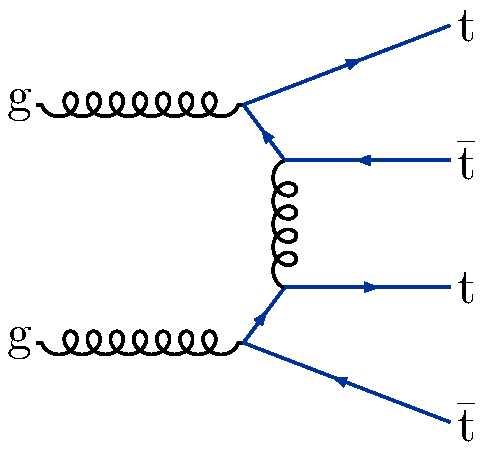
\includegraphics[width=0.35\textwidth]{figs/ftp/ftdiag1.pdf}
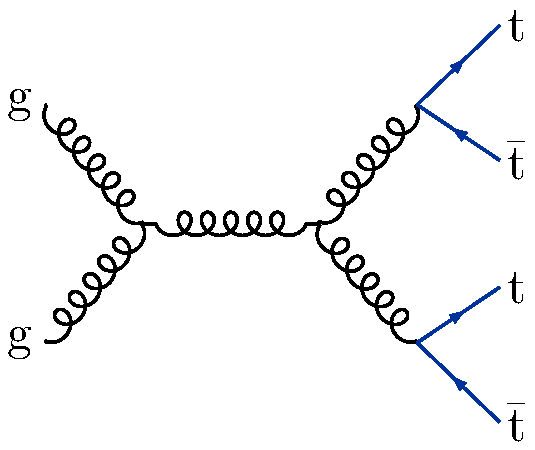
\includegraphics[width=0.35\textwidth]{figs/ftp/ftdiag2.pdf} \\
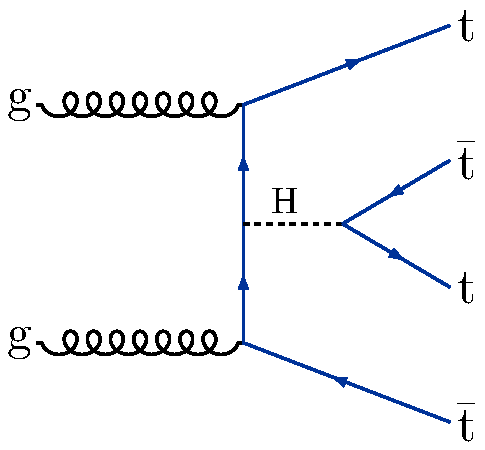
\includegraphics[width=0.35\textwidth]{figs/ftp/ftdiag3.pdf}
\caption{Typical Feynman diagrams for \tttt production at leasting order in the SM.}
\label{fig:ftdiags}
\end{figure}

\subsection{On-shell}

\subsubsection{Two Higgs doublet models}

In the spirit of generality, a simple possible extension of the SM 
is the two Higgs doublet model (2HDM)~\cite{THEORY:Branco2011iw}.
For example, the Minimal Supersymmetric Standard Model (MSSM)
has two Higgs doublets instead of the SM's single doublet.
Two doublets provides for five physical states: 
a light scalar boson $h$, a heavy scalar boson $\PH$, a heavy pseudoscalar boson $\PSA$, and
two charged bosons $\PH^\pm$. Their masses ($m_h, m_\PH, m_\PSA, m_{\PH^\pm}$)
consitute four of the six parameters used in the 2HDM. The other two are $\tan\beta$,
which is the ratio of vacuum expectation values of the two Higgs doublets,
and $\alpha$, which is the rotation angle that diagonalizes the mass matrix of the
two CP-even scalar states $h$ and $\PH$.

Given that observation of a new boson in 2012~\cite{CMS:HiggsObservation,ATLAS:HiggsObservation},
has since been shown to have very SM Higgs-like properties,
there should be a phenomenological constraint on 2HDM theories to
account for this. Fortunately, in a Type-II 2HDM in the alignment limit,
$\sin(\beta-\alpha)\rightarrow 1$,
the CP-even scalar $h$ has
couplings which are SM-like, meaning it can be identified with the particle
discovered, and other states constitute new physics to be discovered.

In Type-II 2HDM, the couplings of the heavy scalar and pseudoscalar to SM
vector bosons are also suppressed, and vanish as
$\cos(\beta-\alpha)\rightarrow 0$. In this limit, production happens mainly
through gluon-fusion. However, the direct search for such new physics via
resonant \ttbar production is hampered by interference with the massive SM
production of \ttbar~\cite{THEORY:Gaemers1984sj,THEORY:Dicus1994bm}. As an
alternative to direct production, since the branching ratio of the heavy
scalar state $\PH$ to up-type quarks (e.g., the top quark) is proportional to
$1/\tan\beta$, at low $\tan\beta$, associated production with three and four
top quark final states provide a relatively clean handle to probe Type-II
2HDM scenarios~\cite{THEORY:Craig2015jba,THEORY:Craig2016ygr}. The one or two top quark
associated production modes are shown in Fig.~\ref{fig:thdm_diagrams}, where
the intermediate heavy boson decays into $\ttbar$ at low $\tan\beta$, resulting in
final states of $\tttt$, $\PQt\bar{\PQt}\PQt\PQq$, and $\PQt\bar{\PQt}\PQt\PW$, respectively.
Heavy boson with masses above twice that of the top quark ($m_{\PH/\PSA}>350\GeV$)
almost exclusively decay into \ttbar.
Thus, a SM search for \tttt would be optimized to directly probe the first of these three final states,
while still retaining sensitivity to the latter two, for sufficiently massive 
scalar and pseudoscalar bosons to allow for on-shell decays into \ttbar.

\begin{figure}[htbp!]
    \centering
    \subfloat[]{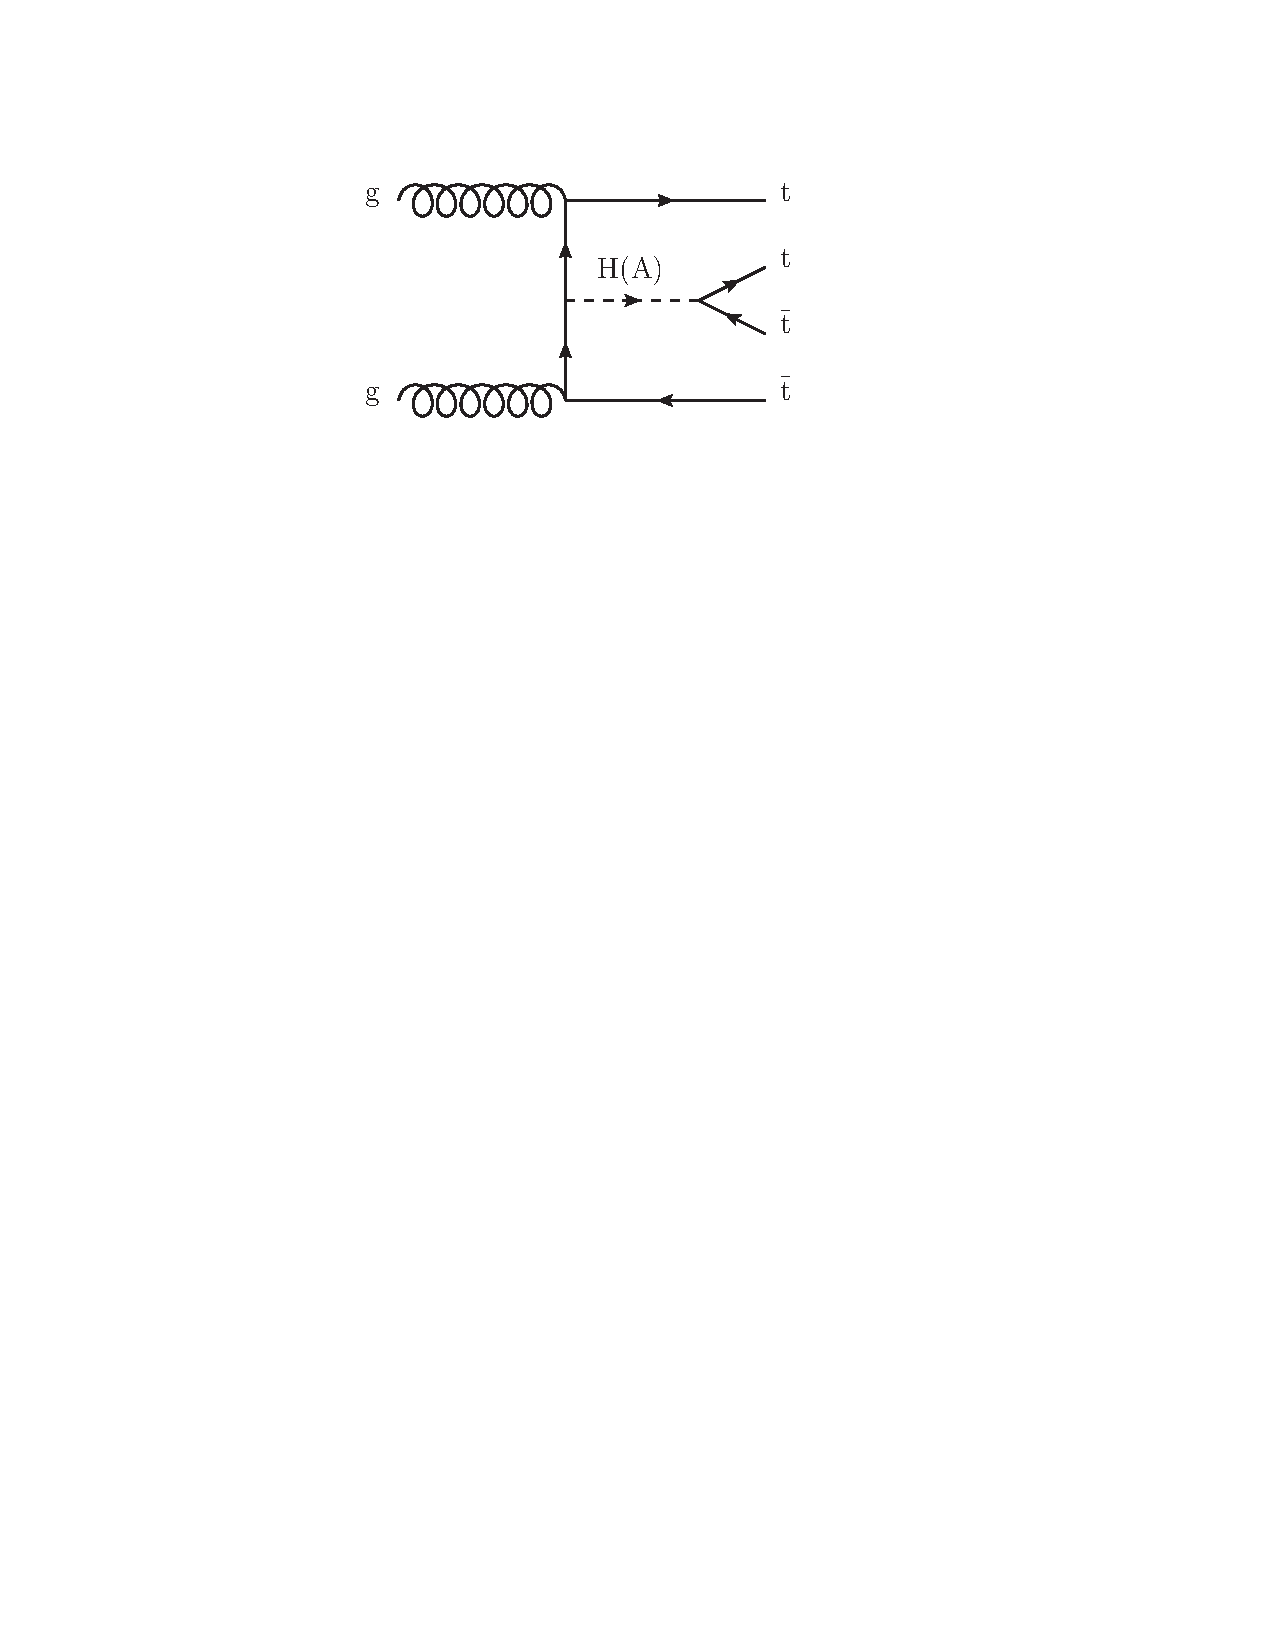
\includegraphics[width=0.40\textwidth]{figs/ftan/bsm_tth_diagram}}
    \subfloat[]{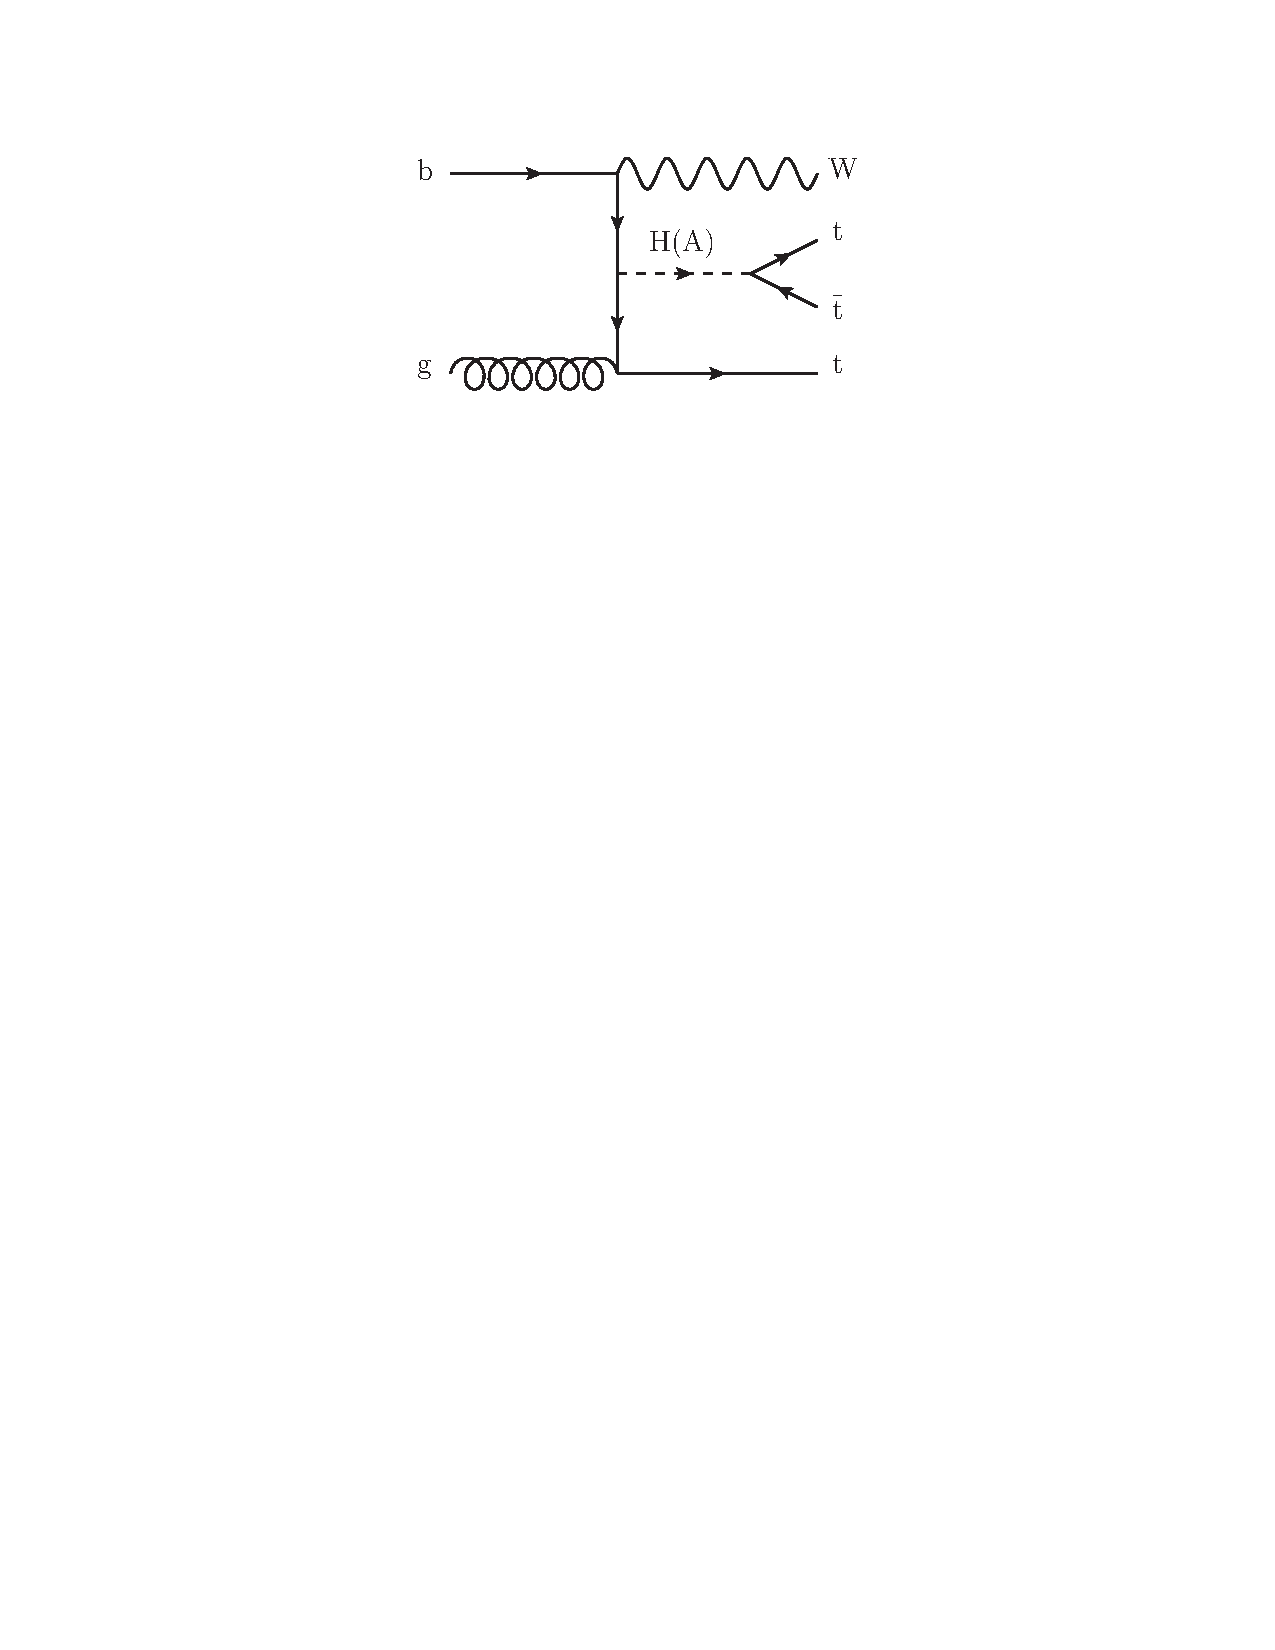
\includegraphics[width=0.40\textwidth]{figs/ftan/bsm_thw_diagram}} \\
    \subfloat[]{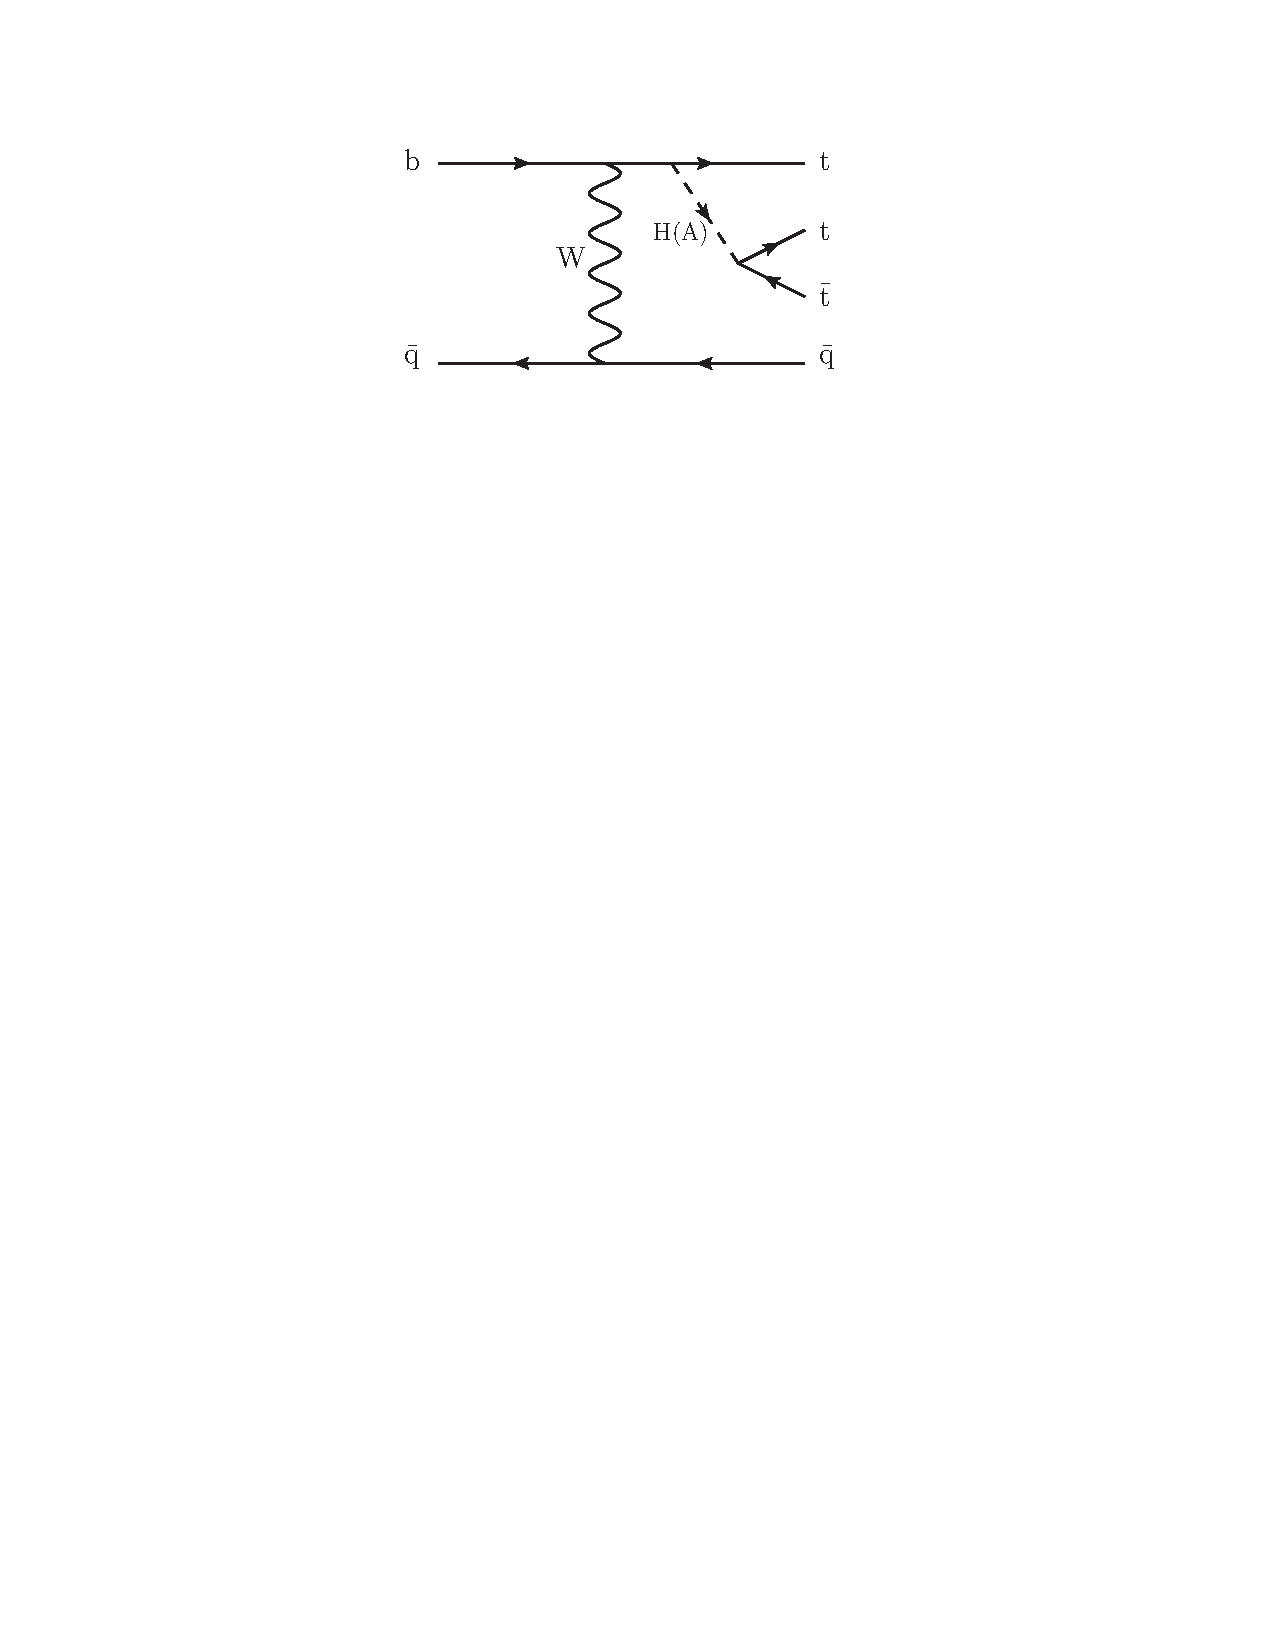
\includegraphics[width=0.40\textwidth]{figs/ftan/bsm_thq_diagram}}
\caption{Diagrams for scalar (pseudoscalar) production in association with 
one or two top quarks.}
\label{fig:thdm_diagrams}
\end{figure}

\FloatBarrier

Leading order cross sections (times branching ratio into \ttbar) for a Type-II 2HDM scenario in the exact alignment limit 
are shown in Fig.~\ref{fig:thdm_2d_xsecs}, as a function of mediator mass and $\tan\beta$.
Processes with $\PH$ and $\PSA$ mediators
are considered separately and the charged bosons $\PH^\pm$ are decoupled by setting their
masses to $10\TeV$. Cross sections are generally slowly falling as a function of increasing mass
and sharply falling for increasing $\tan\beta$. One dimensional cross sections
for three particular values of $\tan\beta$ are shown in Fig.~\ref{fig:thdm_1d_xsec},
and range from approximately 45\ifb at the $2m_\PQt$ threshold to 9\ifb at $m_\PH=650\GeV$
for $\tan\beta=1$.

\begin{figure}[htb!]
    \centering
    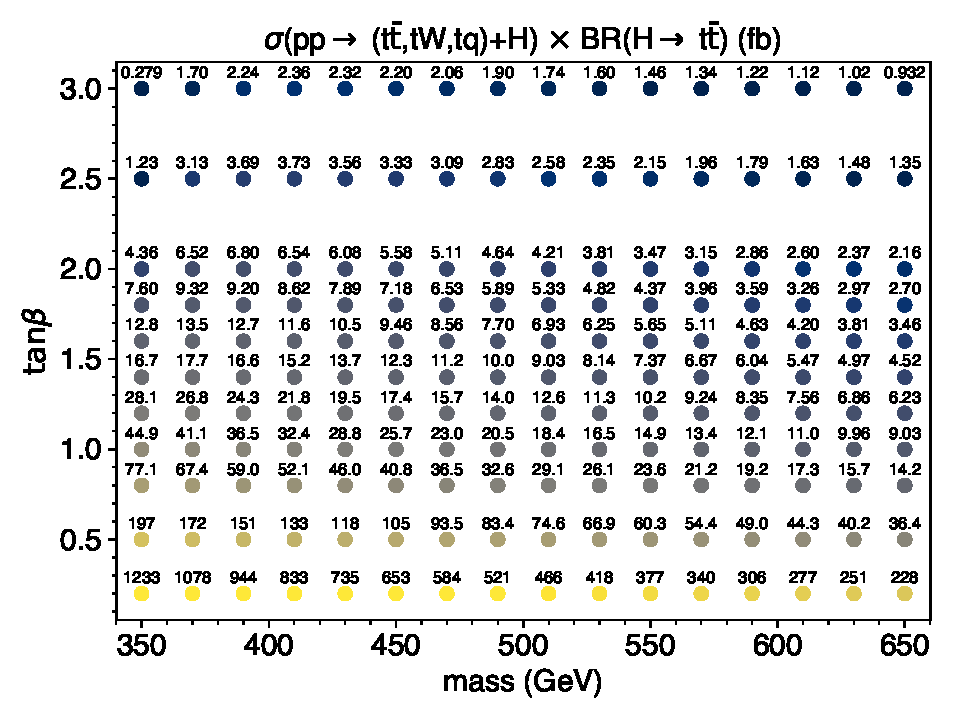
\includegraphics[width=0.75\textwidth]{figs/ftan/plot_2d_2hdm_xsec_h} \\
    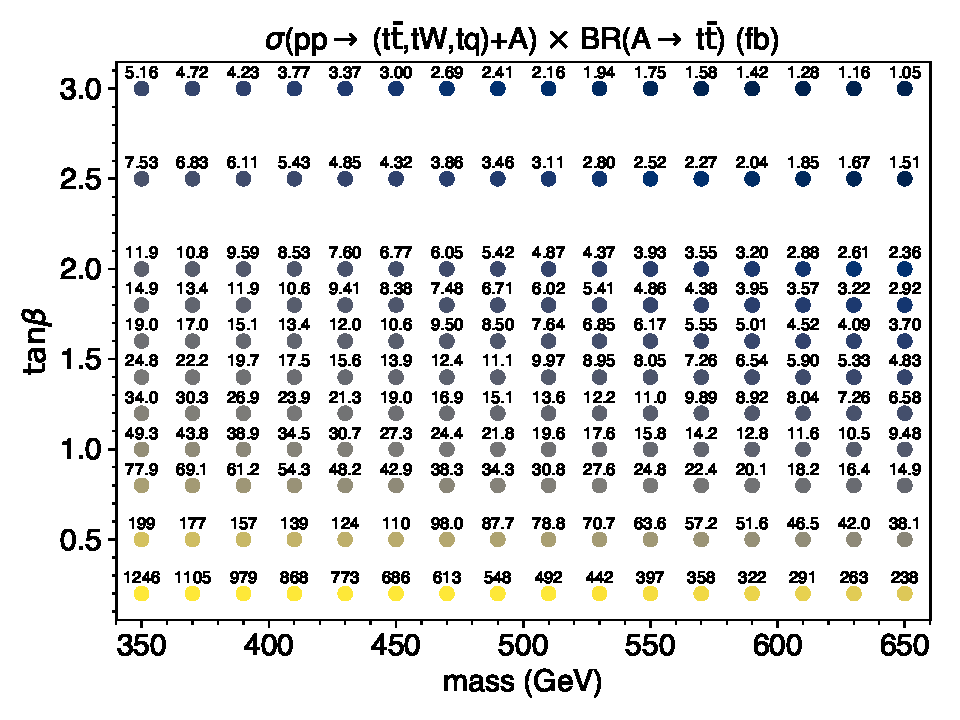
\includegraphics[width=0.75\textwidth]{figs/ftan/plot_2d_2hdm_xsec_a}
\caption{Cross sections times branching ratio into \ttbar for a heavy scalar boson $\PH$ (top) 
or heavy pseudocalar boson $\PSA$ (bottom) as a function of boson mass and $\tan\beta$.}
\label{fig:thdm_2d_xsecs}
\end{figure}

\begin{figure}[htb!]
    \centering
    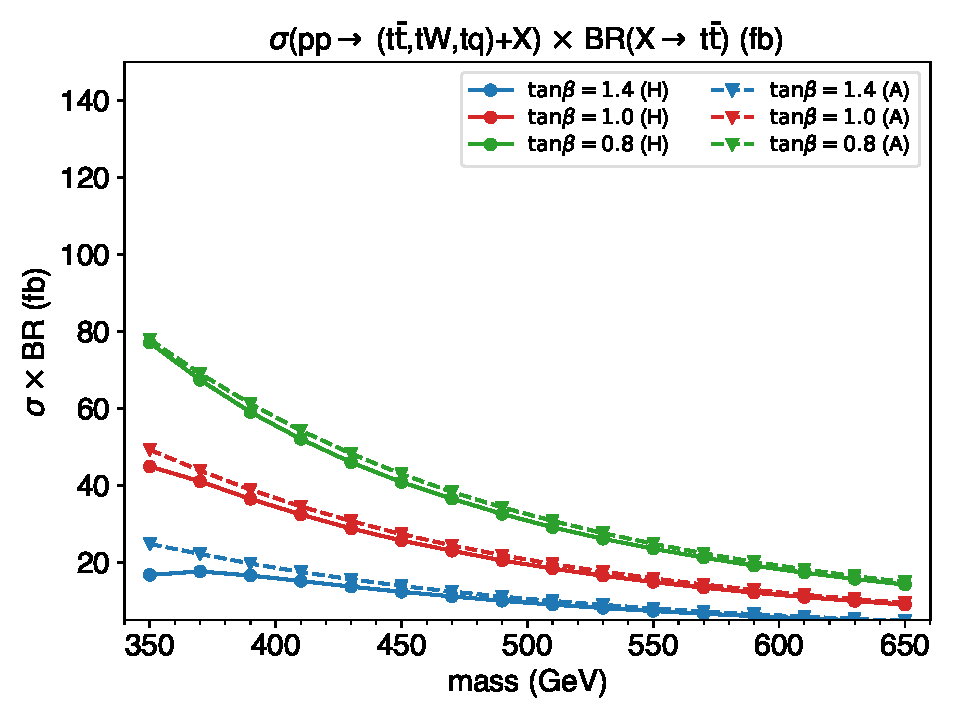
\includegraphics[width=0.75\textwidth]{figs/ftan/plot_1d_2hdm_xsec}
\caption{Cross sections times branching ratio into \ttbar for a heavy scalar boson $\PH$ 
or heavy pseudocalar boson $\PSA$ as a function of boson mass for three assumptions of 
$\tan\beta$ ($0.8, 1.0, 1.4$).}
\label{fig:thdm_1d_xsec}
\end{figure}

\FloatBarrier

\subsubsection{Simplified dark matter models}

Similarly to 2HDM, simplified dark matter (DM) models with scalar or pseudoscalar
mediators decaying into a pair of dark matter or SM particles can be
probed~\cite{THEORY:DMsingletop}. The production of these mediators,
and subsequent decay into invisible dark matter particles,
in association with a one or two top
quarks, was performed by CMS with the 2016 dataset
Ref.\cite{CMS:DMsingletop,CMS:DMttpair}. The production diagrams are shown in
Fig.~\ref{fig:dm_diagrams}.

In the framework of a simplified dark matter model, where the scalar ($\phi$)
or pseudoscalar ($\mathrm{a}$) mediator couples dark matter and SM particles,
the relevant terms of the interaction lagrangian are of the form
\[
    \mathcal{L}_{\phi}=g_{\chi}\phi\bar{\chi}\chi + \frac{g_\mathrm{q} \phi}{\sqrt{2}} \sum_{\mathrm{f}} y_\mathrm{f} \bar{\mathrm{f}} \mathrm{f}
    \quad\quad\quad
    \mathcal{L}_{a}=i g_{\chi}a\bar{\chi}\gamma^5\chi + \frac{i g_\mathrm{q} \mathrm{a}}{\sqrt{2}} \sum_{\mathrm{f}} y_\mathrm{f} \bar{\mathrm{f}} \gamma^5 \mathrm{f}
\]
where $y_\mathrm{f}$ are the fermionic yukawa couplings. The coupling
constants $g_\chi$ and $g_\mathrm{q}$ give the relative strengths of the
mediator coupling to dark matter and SM particles, and are used
interchangeably with $g_\mathrm{DM}$ and $g_\mathrm{SM}$, respectively. The
model has four free parameters ($g_\chi$, $g_\mathrm{q}$, $m_\chi$, and
$m_\mathrm{a}$) which are reduced to two with the assumption of $g_\chi =
g_\mathrm{q} = 1$.

When the mediator mass is above $2 m_\mathrm{t} \approx 350\GeV$, on-shell
decay to \ttbar becomes kinematically accessible, resulting in three or four top
quark final states, so we instead consider a version of the diagrams of
Fig.~\ref{fig:dm_diagrams} with a decay of the mediator into \ttbar rather
than a pair of (invisible) dark matter particles $\chi\bar{\chi}$.
Consequently, the production diagrams and kinematics are identical to those
of the Type-II 2HDM for certain assumptions of mediator mass, dark matter mass,
and $\tan\beta$, and $\phi/\mathrm{a}$ can be identified as $\PH/\PSA$.

In this way, the three or four top quark final states
allow complementarity with the CMS analysis from Ref.~\cite{CMS:DMsingletop} which relied on
a final state with \ttbar and missing transverse energy, provided that
the DM mass is sufficiently large to allow for on-shell decays of the mediator into \ttbar.

The product of cross section and branching ratio of the mediators into \ttbar,
under the assumption of $g_\mathrm{DM}=g_\mathrm{SM}=1$, is shown in 
Fig.~\ref{fig:dm_2d_xsecs}. Note that when $2 m_{\chi}>m_{\PH/\PSA}$,
the decay of the mediators into DM is suppressed in favor of the next-leading mode,
\ttbar, and thus the cross sections become independent of $m_\chi$ above the
marked diagonals. The cross sections at large $m_\chi$ are nearly
identical to those of the 2HDM with $\tan\beta = 1$ shown previously.
However, below the diagonal, the mediator prefers to decay into $\chi\bar{\chi}$
and a search for three or four top quark final states loses sensitivity.

\begin{figure}[htb!]
    \centering
    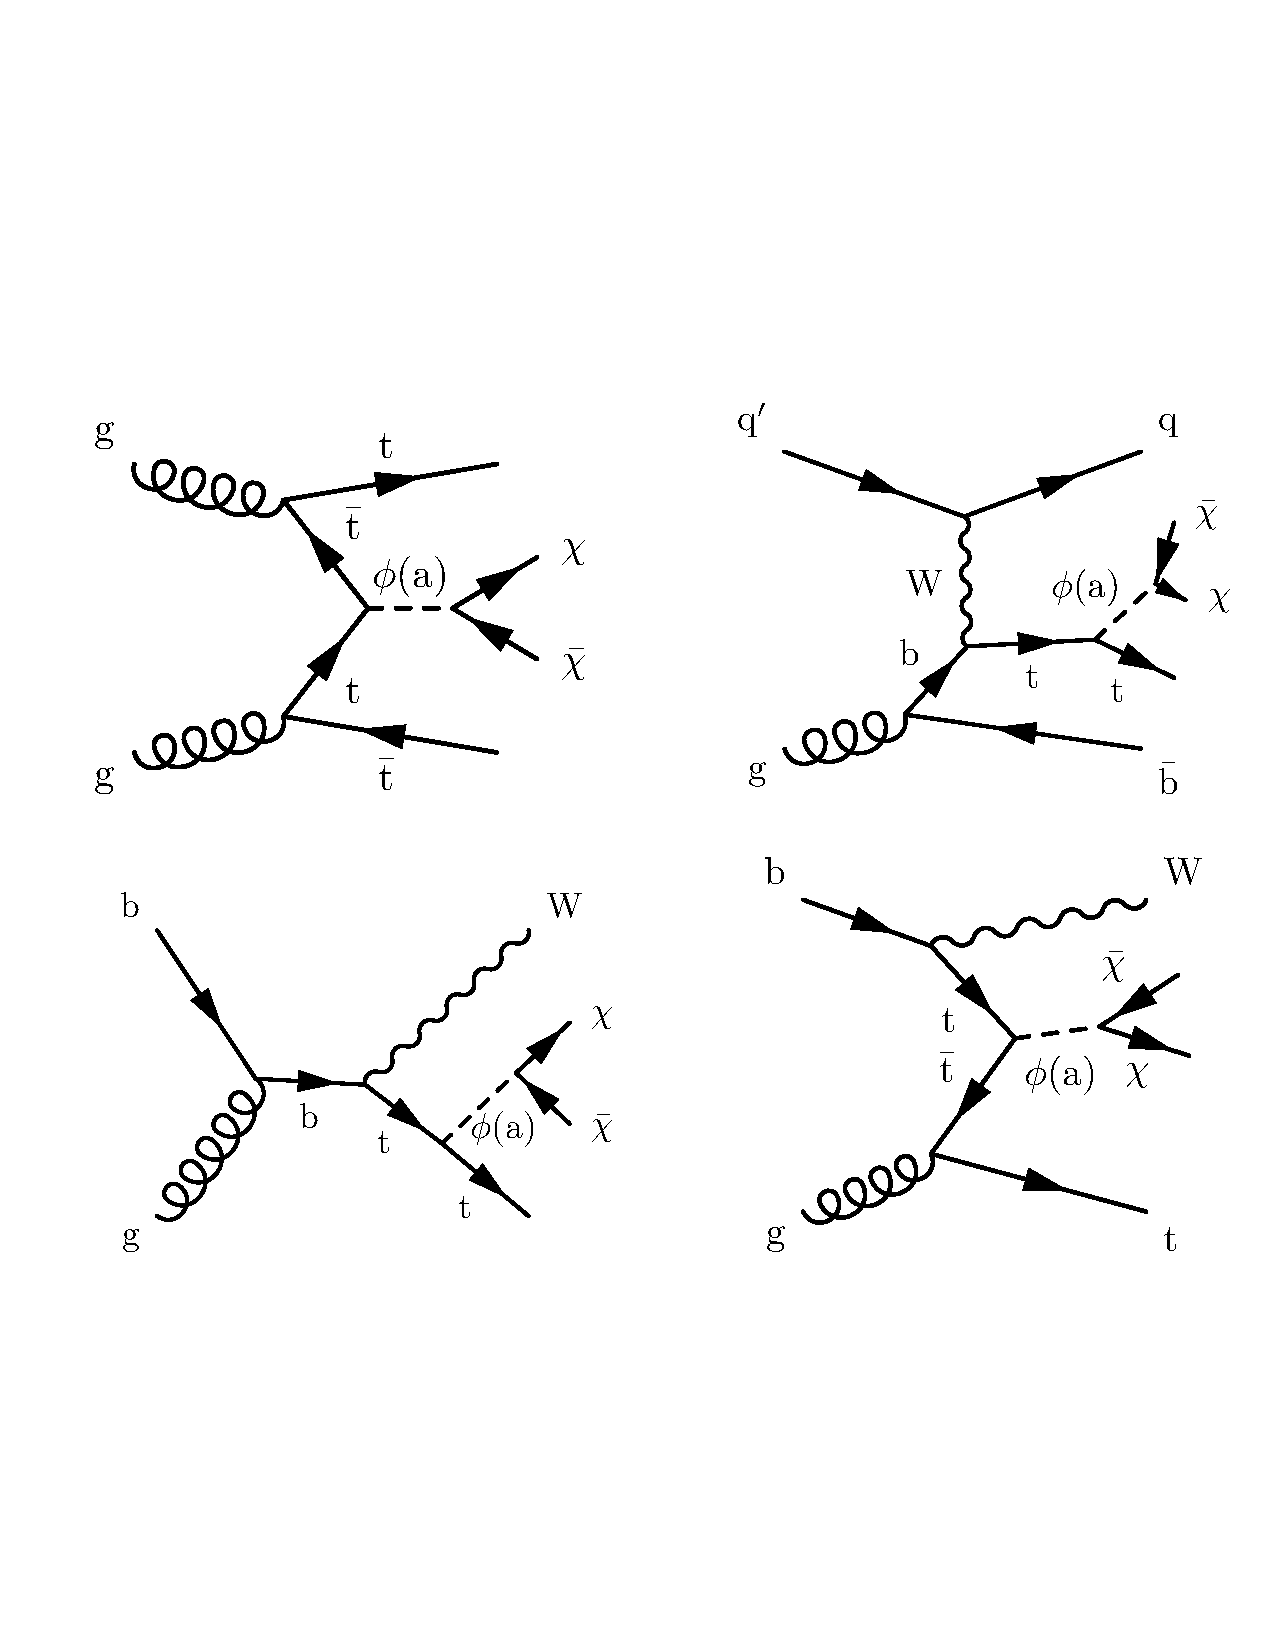
\includegraphics[width=0.75\textwidth]{figs/ftan/bsm_dm_diagrams}
\caption{Diagrams for scalar (pseudoscalar) production in association with a
\ttbar pair (top left), associated t-channel single top (top right),
associated $\PQt\PW$ (bottom row). The mediator subsequently decays into 
a pair of invisible DM particles $\chi\bar{\chi}$.}
\label{fig:dm_diagrams}
\end{figure}

\begin{figure}[htb!]
    \centering
    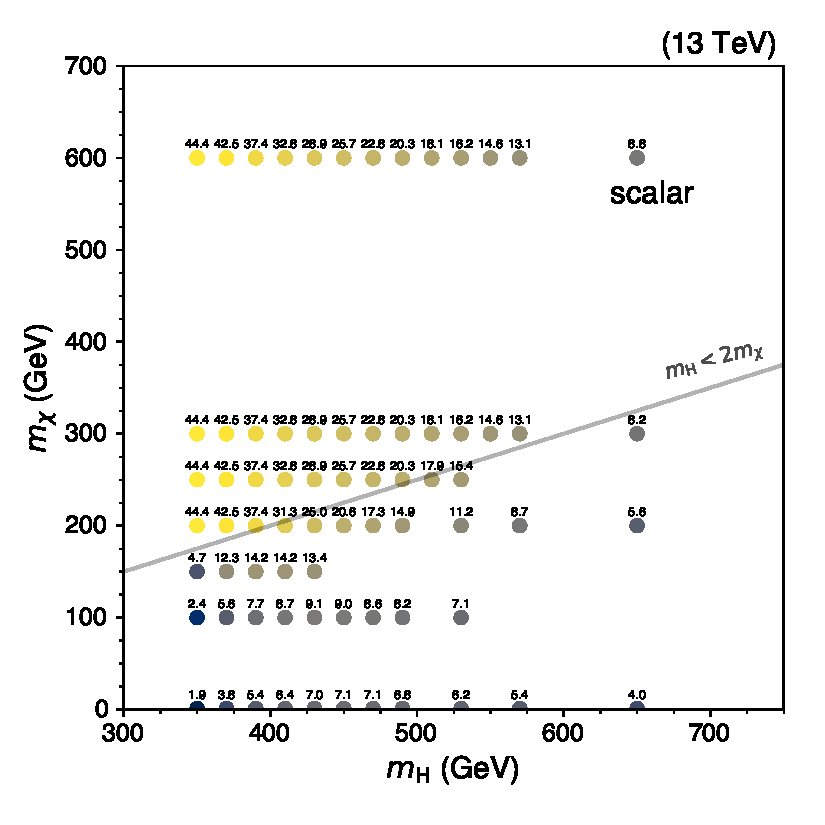
\includegraphics[width=0.60\textwidth]{figs/ftan/plot_2d_dmscalar_xsec_totsm} \\
    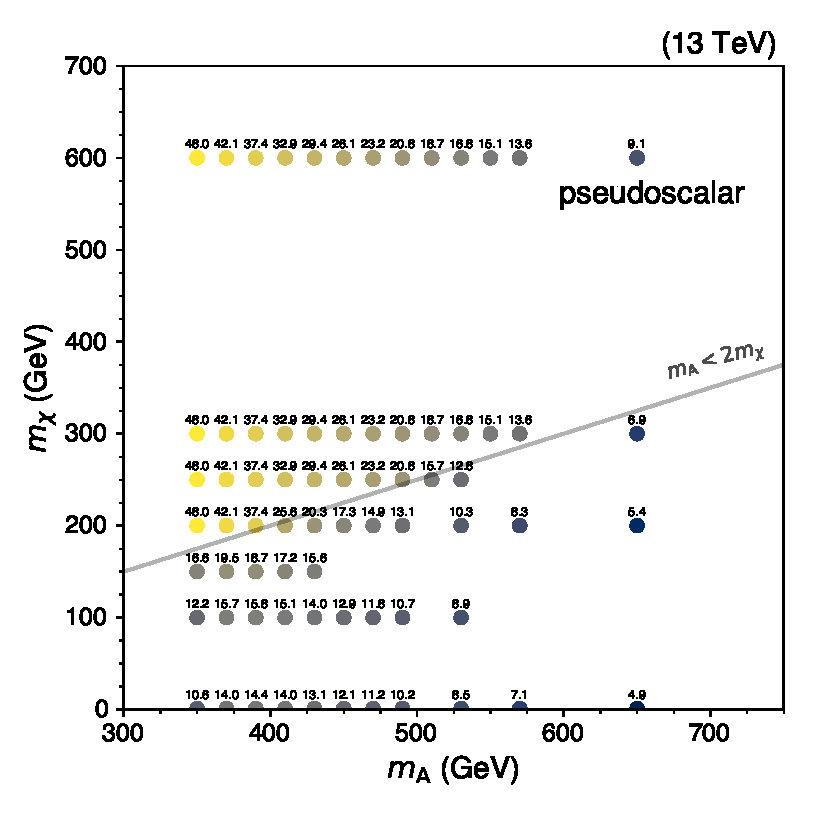
\includegraphics[width=0.60\textwidth]{figs/ftan/plot_2d_dmpseudo_xsec_totsm}
\caption{Cross sections (times branching ratio into $\ttbar$), assuming
$g_\mathrm{DM}=g_\mathrm{SM}=1$, in the plane of $m_\chi$ versus $m_{\PH/\PSA}$ (top/bottom).
}
\label{fig:dm_2d_xsecs}
\end{figure}



\FloatBarrier

\subsection{Off-shell}

\subsubsection{Top quark yukawa coupling}

The SM $pp \rightarrow \tttt$ process includes diagrams with virtual Higgs bosons,
as shown in Fig.~\ref{fig:feynYukawa}. 
The amplitude corresponding to these diagrams is 
proportional to the square of the top Yukawa coupling,
and thus, the cross section of SM \tttt provides
a promising probe into the top Yukawa coupling.

\begin{figure}[!hbtp]
\centering
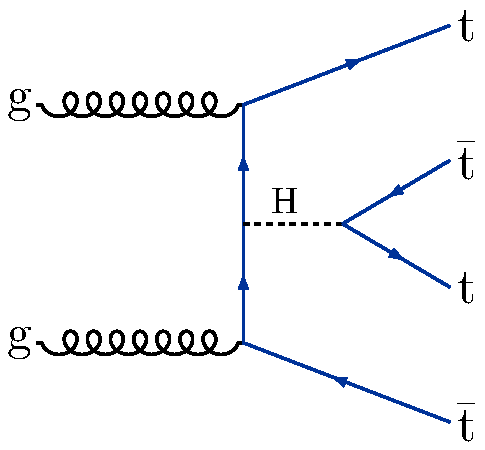
\includegraphics[width=.35\textwidth]{figs/ftp/ftdiag3.pdf} \\
\caption{One of the Feynman diagrams for \tttt including a virtual Higgs.}
\label{fig:feynYukawa}
\end{figure}

Using the notation of Reference~\cite{THEORY:TopYukawaTTTT} the \tttt cross section can be written 
as 

\begin{equation} 
\label{eq:yukawa}
\sigma(\tttt) = \sigma^{\text{SM}}(\tttt)_{g+Z/\gamma} + k_t^4 \sigma^{\text{SM}}(\tttt)_H + k_t^2 \sigma^{\text{SM}}_{\rm int}
\end{equation} 

\noindent where $k_t \equiv y_t/y_t^{\text{SM}}$, $y_t$ is the top Yukawa coupling, and $y_t^{\text{SM}}$ is its SM value.
In equation~\ref{eq:yukawa} the first term on the right hand side corresponds to the 
SM contribution to the cross section from diagrams with gluons or $Z/\gamma$, the second term
is the contribution from diagrams with virtual Higgs bosons, and the third term is the interference between
the two previous terms. Therefore, given a theoretical calculation and a measurement of $\sigma(\tttt)$, one can put 
constraints on $|y_t/y_t^{\text{SM}}|$.

The authors of Reference~\cite{THEORY:TopYukawaTTTT} have calculated the cross section terms at LO.
These are given in Table~\ref{tab:yukawa} and are shown in Fig.~\ref{fig:cross_section_yt},
where the figure shows a curve normalized such that the prediction matches the NLO calculation of 
the \tttt cross section of $12.0^{+2.2}_{-2.5}\unit{fb}$.
The upper and lower values given in Table~\ref{tab:yukawa} correspond to variations
of the renormalization and factorization scale up and down by a factor of two, respectively.

\begin{table} [h!]
\begin{center}
{\renewcommand{\arraystretch}{1.3}
\begin{tabular}{l|ccc}
\hline
   & lower & central & upper \\
\hline
$ \sigma^{\text{SM}}(\tttt)_{g+Z/\gamma}  $ & 14.104 fb & 9.997 fb &  6.378 fb \\
$ \sigma^{\text{SM}}(\tttt)_H $                  & 1.625 fb &  1.167 fb &  0.7655 fb \\
$\sigma^{\text{SM}}_{\rm int} $                   & -2.152 fb &  -1.547 fb &  -0.999 fb \\
\hline
\end{tabular}}
\caption{LO calculation of the terms in equation~\ref{eq:yukawa} from
Reference~\cite{THEORY:TopYukawaTTTT}.  
The uncertainties are from private communications with the authors.}
\label{tab:yukawa}
\end{center}
\end{table}


\begin{figure}[!htbp]
    \centering
    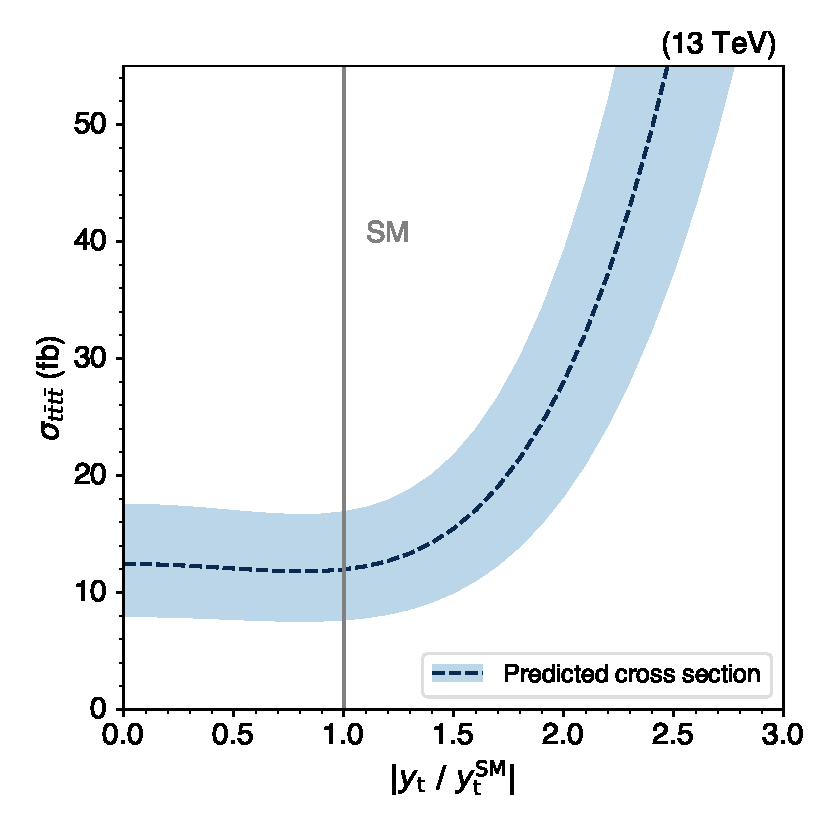
\includegraphics[width=0.75\linewidth]{figs/ftan/cross_section_yt.pdf}
    \caption{
        Predicted \tttt cross section as a function of $|y_t/y_t^{\text{SM}}|$.
    }
    \label{fig:cross_section_yt}
\end{figure}

\FloatBarrier

\subsubsection{Light off-shell mediators}

The production of \tttt may also be influenced by a neutral scalar mediator
($\phi$) or neutral vector mediator ($Z'$) which couple to top quarks and have
masses less than twice the mass of the top quark, distinguishing them from
from similar processes within the 2HDM framework, for example. The off-shell contributions
to the SM \tttt production can be large, as shown in
Ref.~\cite{THEORY:Alvarez2016nrz}. For a large range of masses, the authors have
shown that kinematics are identical when considering these additional
processes, so that the total \tttt cross section is subject to a simple
rescaling.  Corresponding coupling terms in the lagrangian of the form
\begin{equation}
    \mathcal{L}_{Z'}=-g_{t Z'}\bar{t}_R \slashed{Z}' t_R
    \quad\quad\quad
    \mathcal{L}_{\phi}=-g_{t \phi}\bar{t}_L \phi t_R
\end{equation}
There is an approximate independence of kinematics on the coupling strength and mediator mass,
so a single upper limit on the \tttt cross section can be used to place constraints 
on couplings $g_{tZ'}$ and $g_{t\phi}$ as a function of masses $m_{Z'}$ and $m_{\phi}$,
respectively.
Cross sections of \tttt (normalized to SM) as a function of $g_{tZ'}$ 
and $g_{t\phi}$, for different assumptions of $m_{Z'}$ and $m_{\phi}$,
are shown in Fig.~\ref{fig:cross_section_zprimephi}. To illustrate a particular example,
the horizontal dotted line in the figures represents excluding cross sections more than
double that of the SM. These are translated into exclusions on $g_{tZ'}$ and $g_{t\phi}$
via crossing points that are projected onto the x axis.

\begin{figure}[!htbp]
    \centering
    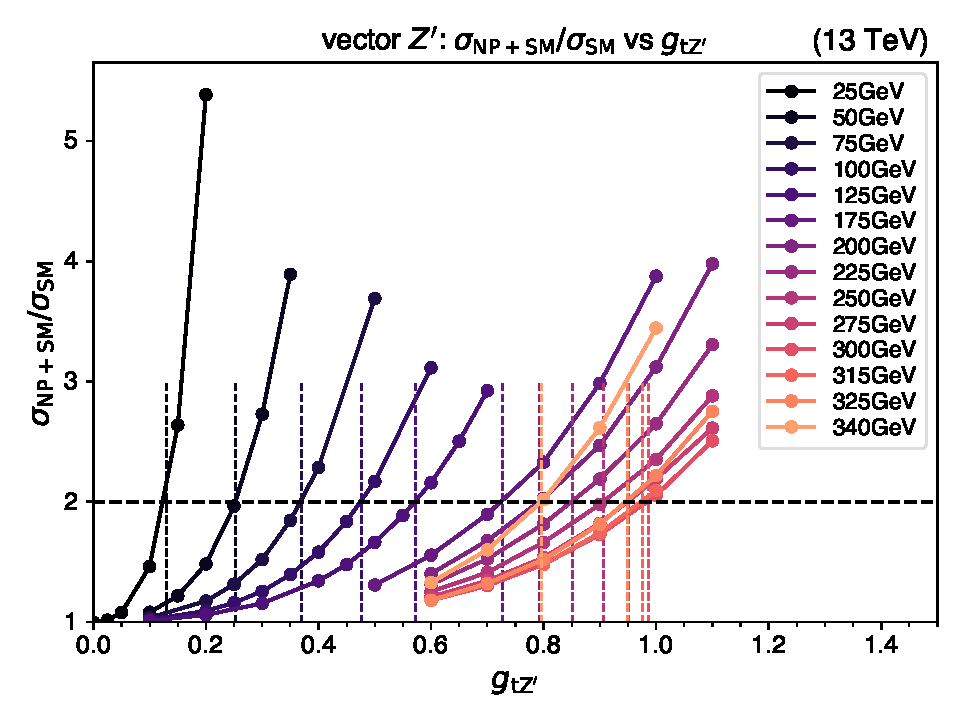
\includegraphics[width=0.78\linewidth]{figs/ftan/plot_xsec_zprime.pdf} \\
    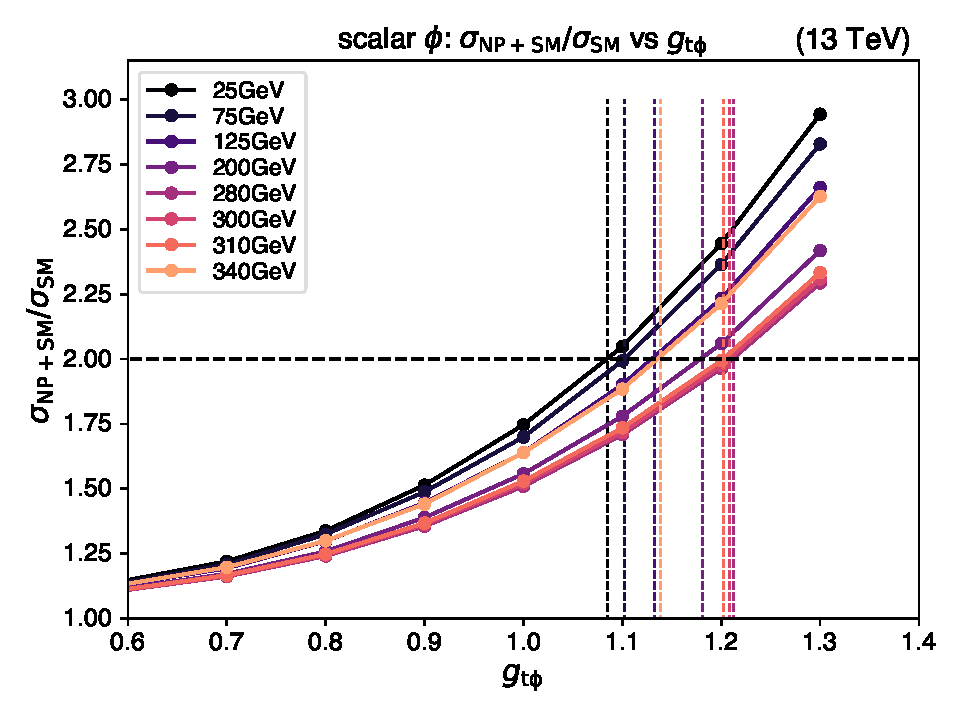
\includegraphics[width=0.78\linewidth]{figs/ftan/plot_xsec_phi.pdf}
    \caption{
        Cross sections of \tttt (normalized to SM) as a function of $g_{tZ'}$ (upper)
        and $g_{t\phi}$ (lower) for different assumptions of $m_{Z'}$ and $m_{\phi}$,
        respectively.
    }
    \label{fig:cross_section_zprimephi}
\end{figure}

\FloatBarrier

\subsubsection{Oblique Higgs parameter}

In a universal effective field theory framework, the Higgs oblique
parameter $\hat H$, defined as the Wilson coefficient of the dimension-6
operator modifying the Higgs boson propagator, can result in deviations of the
SM \tttt cross section, as shown in Ref.~\cite{THEORY:ObliqueHiggs2019}.  These
(off-shell) deviations can be constrained to a level which is competitive with
constraints from on-shell processes.

The two main characteristic effects of this oblique parameter are
an additional term in the SM Higgs boson propagator
\begin{equation}
    P_h(p^2)\approx\frac{i}{p^2-m_h^2}-\frac{i\hat{H}}{m_h^2},
\end{equation}
and a rescaling of the fermionic higgs
couplings
\begin{equation}
    \kappa_f = 1-{\hat H}.
\end{equation}

Using the latest combined fits from the ATLAS experiment for the (on-shell) fermionic couplings,
with 80$\mathrm{fb}^{-1}$ of 13TeV data, the authors of Ref.~\cite{THEORY:ObliqueHiggs2019} find a constraint on
the oblique parameter of $\hat{H} < 0.16$ at 95\% CL.

The authors also calculate that the cross section of (off-shell) \tttt is subject to a fractional modification (with respect to the SM cross section)
at 14 TeV, given by,
\begin{equation}
    \frac{\sigma_{\hat{H}+\mathrm{SM}}}{\sigma_\mathrm{SM}} = 1 + 0.03\left(\frac{\hat{H}}{0.04}\right) + 0.15\left(\frac{\hat{H}}{0.04}\right)^2.
\end{equation}
For an oblique parameter value of 0.1, the formula predicts a doubling of the SM cross section of \tttt.

The SM model within the MadGraph~\cite{THEORY:MADGRAPH5} generator was modified to take into account the extra term in the propagator, as
well as the rescaling of the top-yukawa coupling, and the calculation is repeated
at 13\TeV. The resulting curve is shown in Fig.~\ref{fig:higgs_oblique_madgraph}.

When searching for SM \tttt and placing upper limits on the production cross
section, one can use the relative size of the upper limit with respect to
the SM prediction to exclude $\hat{H}$ values above a threshold. For example,
excluding cross sections more than double that of the SM, $\hat{H}$ values
above approximately 0.14 can be excluded. There are two important caveats
that will need to be taken into account when performing an interpretation for
$\hat{H}$. First, the kinematics of $\tttt$ will be slightly different
depending on the value of $\hat{H}$. Second, the SM process $\ttH$, which is
relevant for the $\tttt$ search, is proportional to
$y_\mathrm{t}^2=(1-\hat{H})^2$ ($\approx 0.74$ at $\hat{H}=0.14$).

\begin{figure}[!htbp]
    \centering
    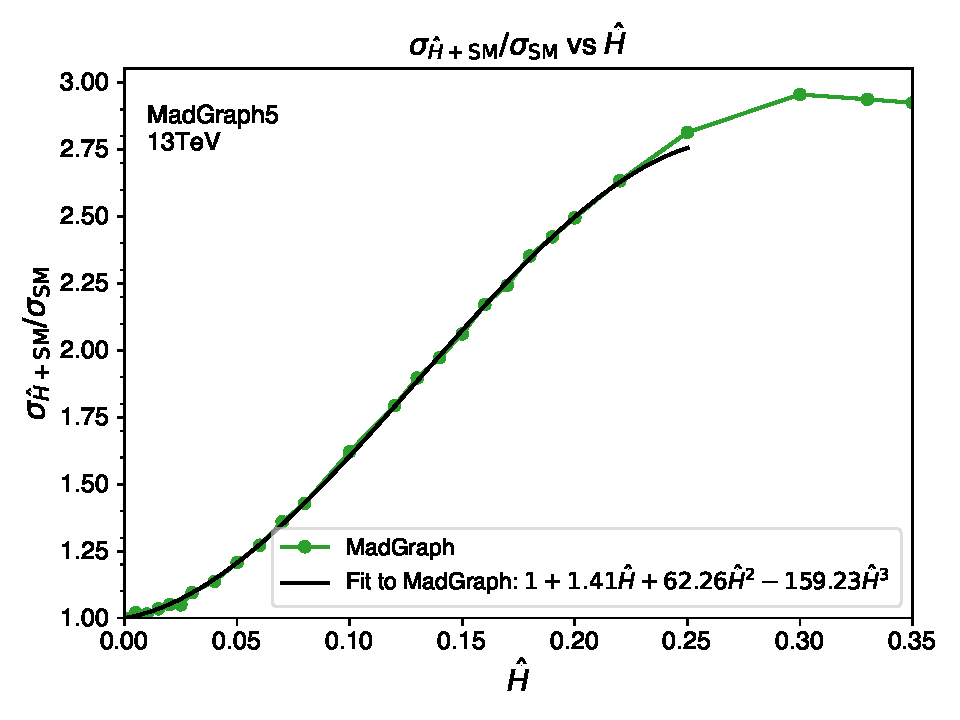
\includegraphics[width=0.75\linewidth]{figs/ftan/higgs_oblique.pdf}
    \caption{
        Cross section (normalized to SM) as a function of oblique parameter $\hat{H}$.
        The green curve is a calculation from MadGraph at 13TeV, and
        the solid black curve is a cubic fit to the calculation.
    }
    \label{fig:higgs_oblique_madgraph}
\end{figure}